\documentclass[../HFT-main.tex]{subfiles} % NEW VERSION IS CASE.tex

%\title{Ethernet Bivalent Repeaters to Æthernet Octavalent Repeaters}
\title{From Bivalent to Octavalent Repeaters}

\begin{document}

\section{Repeaters: from Ethernet to Æthernet}

\begin{marginfigure}
  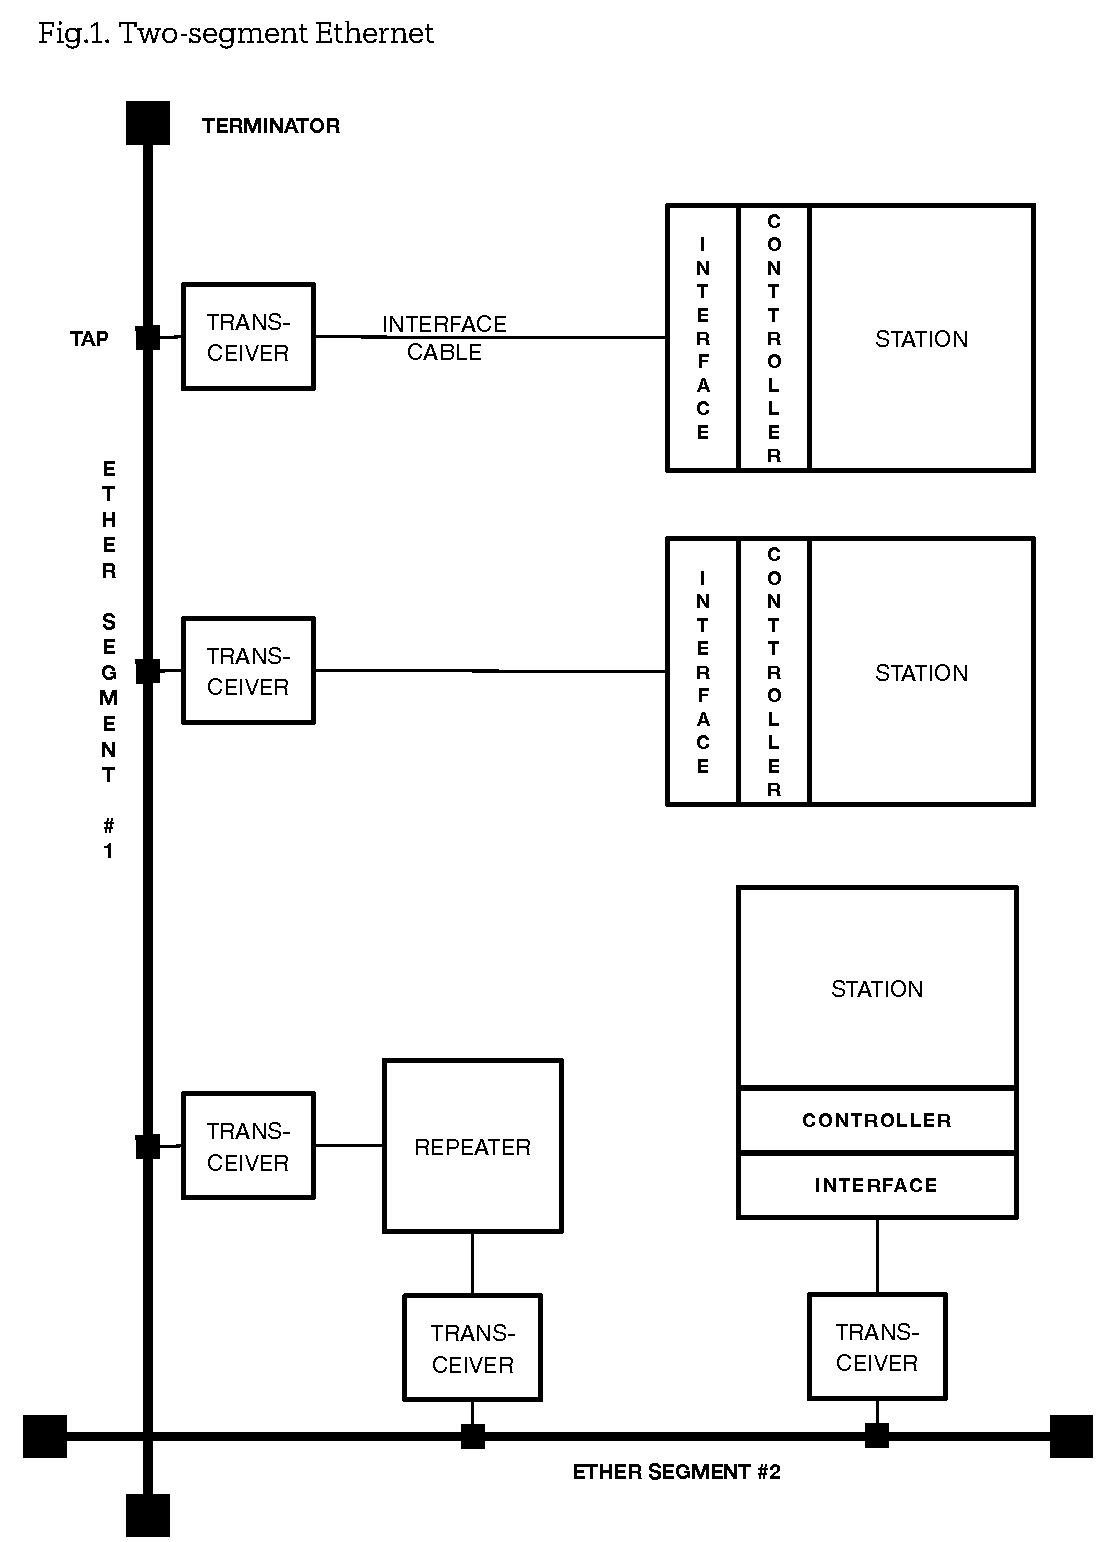
\includegraphics[width=1.1\linewidth]{../../FIGURES/Omni-Figure-1.pdf}
  \caption{Ethernet: REPEATER and TRANSCEIVER (\emph{not} Switch or Router)}
    \vspace{10pt}
\end{marginfigure}

\section{From PHYSICAL Beachfront to Logical Channels}
\begin{marginfigure}
  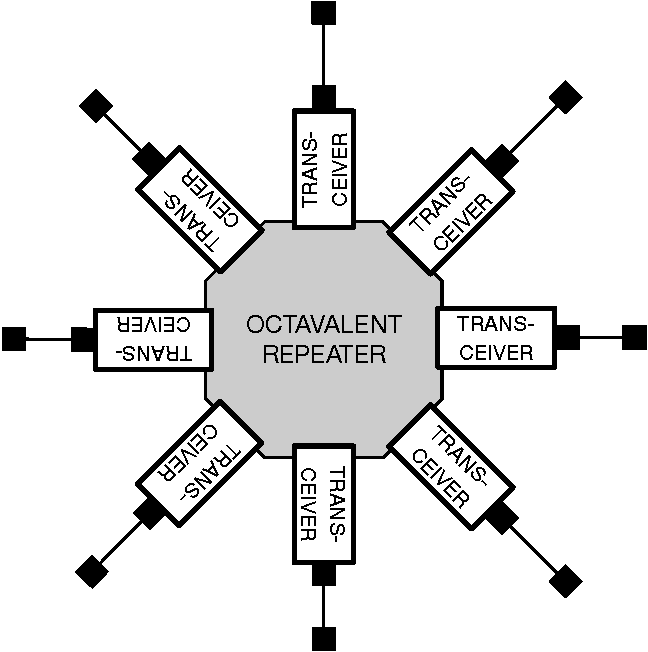
\includegraphics[width=\linewidth]{../../../FIGURES/Octavalent-repeater.pdf} % Odd - this folder address should be the same as the on ebelow
  \caption{\textbf{Physical} Ethernet Bivalent Repeater to Æthernet Octavalent Repeater}
  \vspace{10pt}
\end{marginfigure}

The physical architecture is designed to optimize silicon manufacturing processes. Whole wafers can be use their area more efficiently when the chip connectivity architecture is Hexagonal or Octagonal. This maximizes beachfront connectivity on each chip, and provides logical ``faces'' for connectivity in all 8 directions.

\section{LINKS are CHANNELS}

Æthernet Links are RELIABLE. They do not drop packets we respond to a failure on the link by failing the link and switching ATOMICALLY  to another Link.  More precisely, they maintain the completion of bipartite signaling, like NVLink, Fibrechannel and every other kind of "channel". They are FAIL-STOP, they won't continue to propagate pollution to the data structures in the rest of the system.

This is only possible because logical infrastructure algorithms in the XPUs do failover with \emph{local} information only.


\section{The difference between REPEATERS}

\begin{description}
\item [REPEATERS] Scouting not Routing: Algorithmic forwarding only.  No insecure broadcast or L2 Learning behavior. 
\item [SWITCHES] Build global trees through all the L2 Switches they can find.  Any destination address they don't have in their forwarding table is `broadcast' all the ports.  The port that replies becomes default direction to find that destination in the future.
\item [ROUTERS] Route at Layer 3 (e.g. BGP)
\item [DIRECTORS] For Fibrechannel [add description]
\end{description}

\section{Extending the original Ethernet Concept of REPEATER}
\begin{marginfigure}
  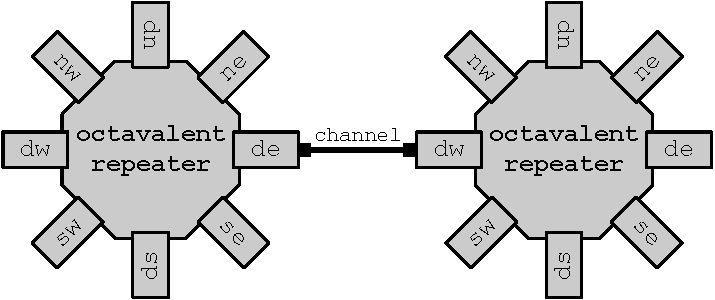
\includegraphics[width=1.2\linewidth]{../../FIGURES/Oct-repeater.pdf}
  \caption{\textbf{Logical}: Æthernet  Octavalent XPU Repeater}
\end{marginfigure}


While switches and routers require extensive administrative attention to configure, reconfigure and debug, Æthernet repeaters are designed to be completely auto-configuring, and auto-healing.  No human attention required.  The physical infrastructure can be configured by an equation  for half-duplex (on each of two channels), or full duplex with each channel having a direction from TX $\rightarrow$ RX.  These channel configurations can also be dynamically reconfigured to adapt to changing workload patterns, and tenant allocation of resources.

\marginnote{The forwarding tables in REPEATERS is programmed by ANT and BEE scouts.  These scouts are severely limited in their range. They do not build global routing information, only LOCAL.}



\clearpage

\section{Octavalent (Compass Point) Scouting} %- THIS APPEARS TO BE DUPLICATE WITH WHATS IN TOPOLOGY.TEX}
\begin{marginfigure}
  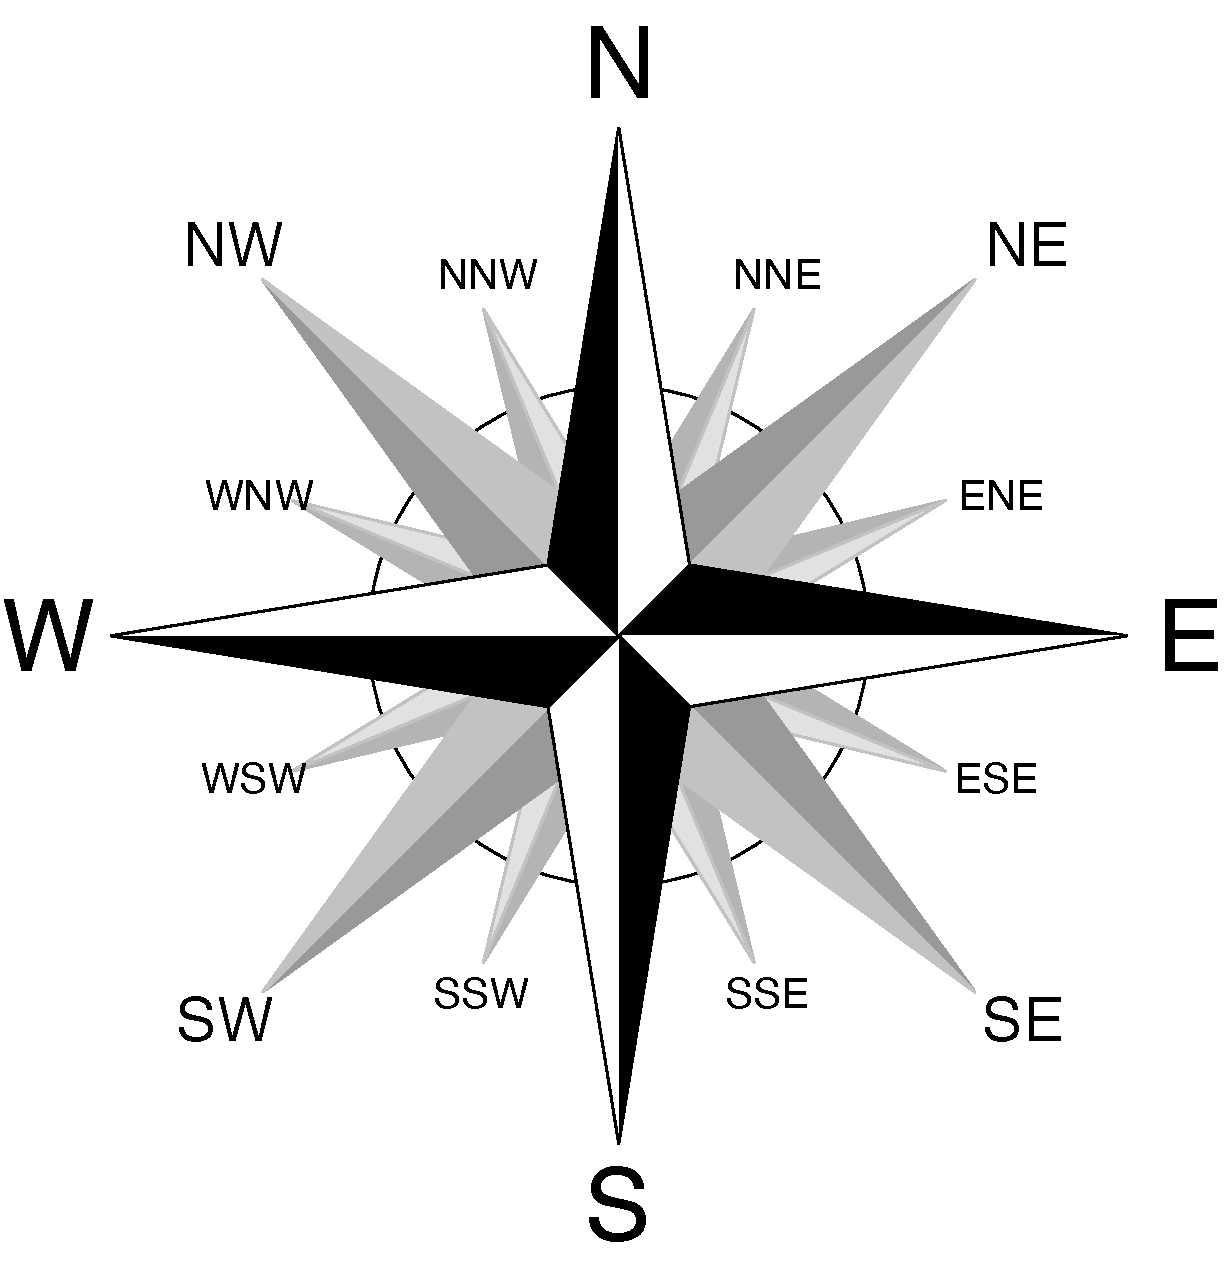
\includegraphics[width=\linewidth]{../Figures/Compass-Rose.pdf}
  \caption{Compass Point Scouting on octavalent nodes with 8 primary (outgoing) and 8 secondary (incoming) --  total 16 configurable TX/RX channels on each port (direction)}
\end{marginfigure}

Every Cell (XPU) with 8 reconfigurable ports will discover its environment.


\section{Biologically Inspired “Scouting” \emph{not}  “Routing”}

Each of these 8 ports has 2 connections (transmit, receive, swap). Although the Chiplet Ethernet specification allows for initial configuration and reconfiguration of these to be used for other purposes, and for dynamic reconfiguration. We specify \emph{scouting} protocols as a precursor discovery protocol, and underneath \emph{routing} described later  

Because any absolute cartesian naming scheme cannot scale, is brittle (to errors and reconfigurations) we use a relative addressing scheme for the scouts (Ants, Bees), for each cell to independently discover its environment. 

Scouts  therefore use \emph{source} routing, where the path explored is pre-determined. As in the case of Ants, these directions can be random. They leave a pheromone trail so they can find their way back home.  In Æthernet clusters, Ants can have other kinds of exploratory behaviors, such always turning right or always turning left, to explore the neighborhood in a circular fashion. 

These kind of mechanisms have already been explored in the literature, and is known as deflection or bufferless routing. 

\section{Connection with bufferless and deflection routing}

Below is an overview of how biologically inspired “scouting” or “discovery” mechanisms connect with key ideas in bufferless (hot-potato) routing and deflection routing, especially in mesh-like topologies where routers have ports arranged along the cardinal (N, E, S, W) and intercardinal (NE, SE, SW, NW) directions. Although the terminology and details vary across papers, the essential themes can be traced in both NoC (Network-on-Chip) and larger-scale interconnection network literature.

%\begin{enumerate}

\subsection{Local decisions and emergent global organization}


\begin{itemize}
\item Scouting/Discovery Phase: Biologically inspired methods (e.g., ant-colony-inspired or pheromone-based algorithms) often employ “scout” packets or “explorer” agents that roam the network. These scouts collect local congestion or path-quality information and deposit some form of “trail” (akin to pheromones).
\item Emergent Routing Table Updates: Each router or switch updates local routing information (sometimes called a local “pheromone table”). Over time, paths that prove consistently “good” get reinforced; less efficient paths fade. This local, probabilistic approach can converge on globally efficient routes with no central coordination.
\end{itemize}



\subsection{Relevance to On-Chip or 2D Mesh Topologies}

 


\begin{itemize}
\item Local Compass Directions: In a regular mesh (e.g., 2D grid) or torus, each router has up to 4 (N, E, S, W) or 8 ports (adding NW, NE, SW, SE). A biologically inspired algorithm can treat each output port as a possible “direction of travel.”
\item Natural Fit for Scouting: The local directional structure matches how “ants” or “foraging agents” might look around in each direction, choosing a route based on local pheromone levels (akin to local congestion or link utilization).
\end{itemize}

Thus, the scouting/discovery mechanism is all about gathering local “pathworthiness” data and then directing future traffic toward better routes—exactly how a local compass-based system can easily be integrated.

\subsection{Bufferless (Hot-Potato) Routing}

\subsection{Basics of Bufferless Routing}

\begin{itemize}
\item No Packet Buffers (or Very Limited Buffers): In a bufferless architecture, every router typically either immediately forwards or deflects each incoming packet. Packets cannot wait in large queues when an output port is congested.
\item Hot-Potato / Deflection Character: When the preferred output port is unavailable, the packet is sent out of a different (less ideal) port—“hot-potato” style—rather than being buffered.
\end{itemize}

\subsection{Connection with Biologically Inspired Approaches}

\begin{itemize}
\item Continuous Movement: Biologically inspired scouts are already designed to wander and discover; in a bufferless system, “wandering” (via deflections) is also central. This synergy means a router can apply a heuristic (like a pheromone table) to pick the “best available port” quickly, but if that port is busy, the packet must choose an alternate direction.
\item Adaptive Reinforcement Over Time: In a bufferless design, a packet cannot linger while waiting for the optimal output. However, local “pheromone” or “congestion” metrics can still help route the majority of packets down better ports more often. Over time, high-traffic edges might become less appealing, guiding packets to less-congested directions.
\end{itemize}

\subsection{3. Deflection Routing}

\subsection{How Deflection Routing Works}

\begin{itemize}
\item Forced Misrouting / Deflection: If the desired or minimal-distance output port cannot be taken (due to contention), the router picks another output. The packet may travel away from its ultimate destination (a “deflection”), but eventually, it should be re-routed back on track.
\item Common in Low- or No-Buffer Architectures: Deflection routing is one way to handle resource contention when buffer space is unavailable.
\end{itemize}

\subsection{Tying It Back to the Compass Ports \texttt{\{DN,NE,DE,SE,DS,SW,DW,NW\}}}

\begin{itemize}
\item Local Prioritization: In an 8-port (or 4-port) router, one can define a strict or heuristic priority among the directions. For example, a packet traveling generally “north-east” might prefer the N or E port if free; if both are busy, it might deflect NE, or in the worst case, deflect NW or SE.
\item Biologically Inspired Ranking: The “pheromone” concept can be used to rank the output directions. The highest “pheromone” port is tried first, then so on down the rank. This effectively merges a local heuristic (pheromone) with forced deflection for whichever ports remain free.
\end{itemize}

In practice, such a scheme allows packets to “scout” and reinforce certain directions while still ensuring that they never have to wait for a blocked port.

\subsection{4. Example Flow in an 8-Port Router}

\begin{enumerate}
\item	Receive a Packet coming in from, say, the south port.
\item	Look Up Destination (or partial coordinate heading). For instance, the packet is trying to reach a node in the north-east region, so N or E might be favored.
\item	Check Local “Pheromone” or Routing Table: Suppose the local pheromone table says port NE is the best guess based on past traffic patterns.
\item	If NE Port Is Free: Forward the packet NE.
\item	If NE Port Is Busy: Check next best local direction (N, E, or NW/SE fallback).
\item	If All Preferred Ports Are Busy: Packet is deflected to any open port (could be even SW in the worst case).
\item	Local Table Update: The router sees how that choice ended up affecting the packet (if it eventually left the region quickly or ended up in a congested area). Over time, these experiences feed back into local pheromone levels.
\end{enumerate}

Despite the forced misrouting (deflections), the biologically inspired feedback approach often keeps net throughput healthy and tries to avoid systematic congestion ``hot spots.''


These resources flesh out how bufferless or deflection routing is implemented (especially in on-chip contexts) and how biologically inspired heuristics can be adapted to local, minimal-knowledge scouting decisions.

\subsection{6. Concluding Remarks}

\begin{itemize}
\item Shared Tenets: Both biologically inspired scouting and deflection-based, bufferless routing rest on local decision making. In biologically inspired schemes, scouting packets “discover” or “reinforce” certain paths. In deflection routing, each router makes a quick (local) decision when a preferred port is blocked, forcing packets to keep moving.
\item Complementary Mechanics: Because biologically inspired “pheromone” updates naturally reflect congestion and path usage, they integrate well with a bufferless or deflection style—turning forced misroutes into valuable “exploration” signals that feed back into local heuristics.
\item Directional Routing: The presence of N, S, E, W (plus diagonals) \texttt{\{DN,NE,DE,SE,DS,SW,DW,NW\}} simply defines how many possible local moves each ANT can attempt as it travels from one cell the the next.  In 2D meshes or tori, these directions make for a convenient $R,\theta$ coordinate system that parallels how ants (or other scouts) might sense local gradients or pheromone intensities in each of eight compass directions.
\end{itemize}

Overall, if we combine a scouting mechanism (to adaptively find neighbors and good routes) with deflection routing (to handle buffer constraints or high contention), we get a dynamic, emergent routing system in which packets flow continuously and local updates shape global traffic patterns in a self-organizing fashion.

All this happens without the need for Source/Destination Addresses, which present severe security problems by exposing the ``identity" of nodes making them vulnerable to attack.

\section{Connection with the Literature}  
\begin{enumerate}
\item  Hot-Potato Routing (Deflection Routing):
	\begin{itemize}
	\item Baran, P. (1962). On Distributed Communications Networks. IEEE Transactions on Communications. (Early ideas of “hot-potato” and distributed routing).
	\item Dally, W., \& Towles, B. (2004). Principles and Practices of Interconnection Networks. (Excellent overview of deflection routing in modern network design).
 	\end{itemize}

\item  Biologically Inspired / Ant-Based Routing:
	\begin{itemize}
	\item Di Caro, G. A., \& Dorigo, M. (1997). AntNet: Distributed stigmergetic control for communications networks. Journal of Artificial Intelligence Research.
	\item Schoonderwoerd, R., Holland, O., Bruten, J., \& Rothkrantz, L. (1996). Ant-based load balancing in telecommunications networks. Adaptive Behavior.
	\end{itemize}
\item	Network-on-Chip with Deflection/Bufferless Approaches:
	\begin{itemize}
	\item Moraes, F. et al. (2004). A Low Area Overhead Packet-switched Network on Chip: Architecture and Prototyping. SBCCI.
	\item Fallin, C., et al. (2012). CHIPPER: A Low-Complexity Bufferless Deflection Router. HPCA.
	\end{itemize}
\end{enumerate}


\section{FAQ}

Q1: (Varun)  What are the fundamental differences between Switches and LINKs and how does the latter improve upon the former?

A1: Switches are pre-distinguished CELLS.   When each CELL is able to forward scout packets, switches are superfluous, and represent unnecessary diversity complexity.  See Document 1 (Exec-Summary-Links.pdf)


A1: The responsibility for guarantees in this Layer 1/2 Protocol is completely within this Æthernet Specification.   Top of Rack (ToR) and other Switches are the Gateway to the L3 world, which we have no control over.  There will be no direct correspondence between the identity and the individuality of CELLS, and the outside world of MAC Addresses, or IP Addresses. This is absolutely necessary to maintain the security guarantees.

\end{document}
